\chapter{Result}
\label{chp:result}
\section{Overview}
\label{result:overview}
This chapter presents comprehensive evaluations of the FlatCityBuf format, demonstrating its performance characteristics and practical applicability through multiple assessment approaches. The evaluation encompasses both technical performance metrics and real-world implementation scenarios to provide a holistic understanding of the format's capabilities.

The chapter is structured around several key evaluation components. First, a web prototype implementation is presented to demonstrate FlatCityBuf's practical capabilities in browser environments, showcasing how the format enables partial data access for large 3D city models through HTTP Range Requests.

Second, the datasets used throughout the evaluation are described, including both the established benchmark datasets from \citet{ledoux_2024} and additional PLATEAU datasets from the Takeshiba district of Tokyo, providing context for the performance comparisons and ensuring reproducibility of results.

Third, file size comparisons are conducted across different encoding formats to evaluate storage efficiency and compression characteristics of FlatCityBuf relative to existing CityJSON variants.

Finally, web environment evaluations demonstrate real-world performance characteristics by measuring data retrieval times and network efficiency in browser-based scenarios. These tests specifically evaluate the effectiveness of HTTP Range Requests for selective data access, providing insights into bandwidth optimisation and response times critical for web-based 3D city model applications.

The following sections present detailed results from each evaluation component, culminating in integrated analyses that synthesise findings to provide comprehensive insights into FlatCityBuf's performance characteristics and practical benefits for 3D city model applications.

\subsection{Web Prototype}
\label{result:web_prototype}

\subsection{Cross-Platform Implementation}
\label{result:cross_platform_implementation}

FlatCityBuf provides range request capabilities across multiple platforms to maximise accessibility and integration options:
\subsubsection{Cross-Platform Support}
\label{result:cross_platform_implementation:cross_platform}

FlatCityBuf is implemented primarily as a Rust library that can be used in both native environments and web browsers. The same codebase is compiled to:

\begin{itemize}
  \item Native Rust library for server-side applications and desktop GIS tools
  \item \ac{wasm} module for browser-based applications with JavaScript interoperability
\end{itemize}

This cross-platform approach enables FlatCityBuf to work with both Rust's native HTTP clients and browser-based Fetch \ac{api} implementations. The \ac{wasm} implementation has one notable limitation: current browser \ac{wasm} implementations use a 32-bit memory model (4GB limit), which may constrain processing of country-level datasets. This limitation will be resolved with the upcoming \ac{wasm} Memory64 proposal \citep{WebAssemblyCoreSpecification2}.
\subsubsection{Web prototype}
\label{result:cross_platform_implementation:web_prototype}

To demonstrate FlatCityBuf's capabilities in web environments and illustrate practical user interactions with the data, a functional web prototype was developed. The prototype is publicly accessible at \url{https://fcb-web-prototype.netlify.app/}. It leverages the WebAssembly module of FlatCityBuf combined with TypeScript and React for the frontend implementation, with Cesium serving as the 3D map rendering engine.

The prototype operates on a substantial dataset covering approximately 20km $\times$ 20km of South Holland, Netherlands, stored as a single 3.4GB FlatCityBuf file. This file is delivered directly from Google Cloud Storage\citep{gcs}, a serverless storage service, where it exists as a static file similar to images or videos, requiring no specialized server-side processing. Despite this large file size, the application remains responsive by utilising the HTTP range request capabilities described in \autoref{result:cross_platform_implementation:cloud_integration}. Users can interact with the data through several query mechanisms:

\begin{itemize}
  \item \textbf{Spatial queries}: Users can filter features either by defining a spatial bounding box or by placing a point on the map to retrieve features based on intersection or nearest-neighbor relationships.

  \item \textbf{Attribute queries}: The interface supports filtering features through attribute conditions (\eg, \texttt{building id = 1, height > 10m}), demonstrating the attribute index capabilities.

  \item \textbf{Data export}: Users can download the filtered subset of features in CityJSONSeq format, showcasing the format conversion capabilities.
\end{itemize}

This prototype effectively demonstrates how FlatCityBuf enables browser-based applications to work with large 3D city models without downloading the entire dataset, providing responsive performance even on consumer-grade hardware and network connections.

\begin{figure}[ht]
  \centering
  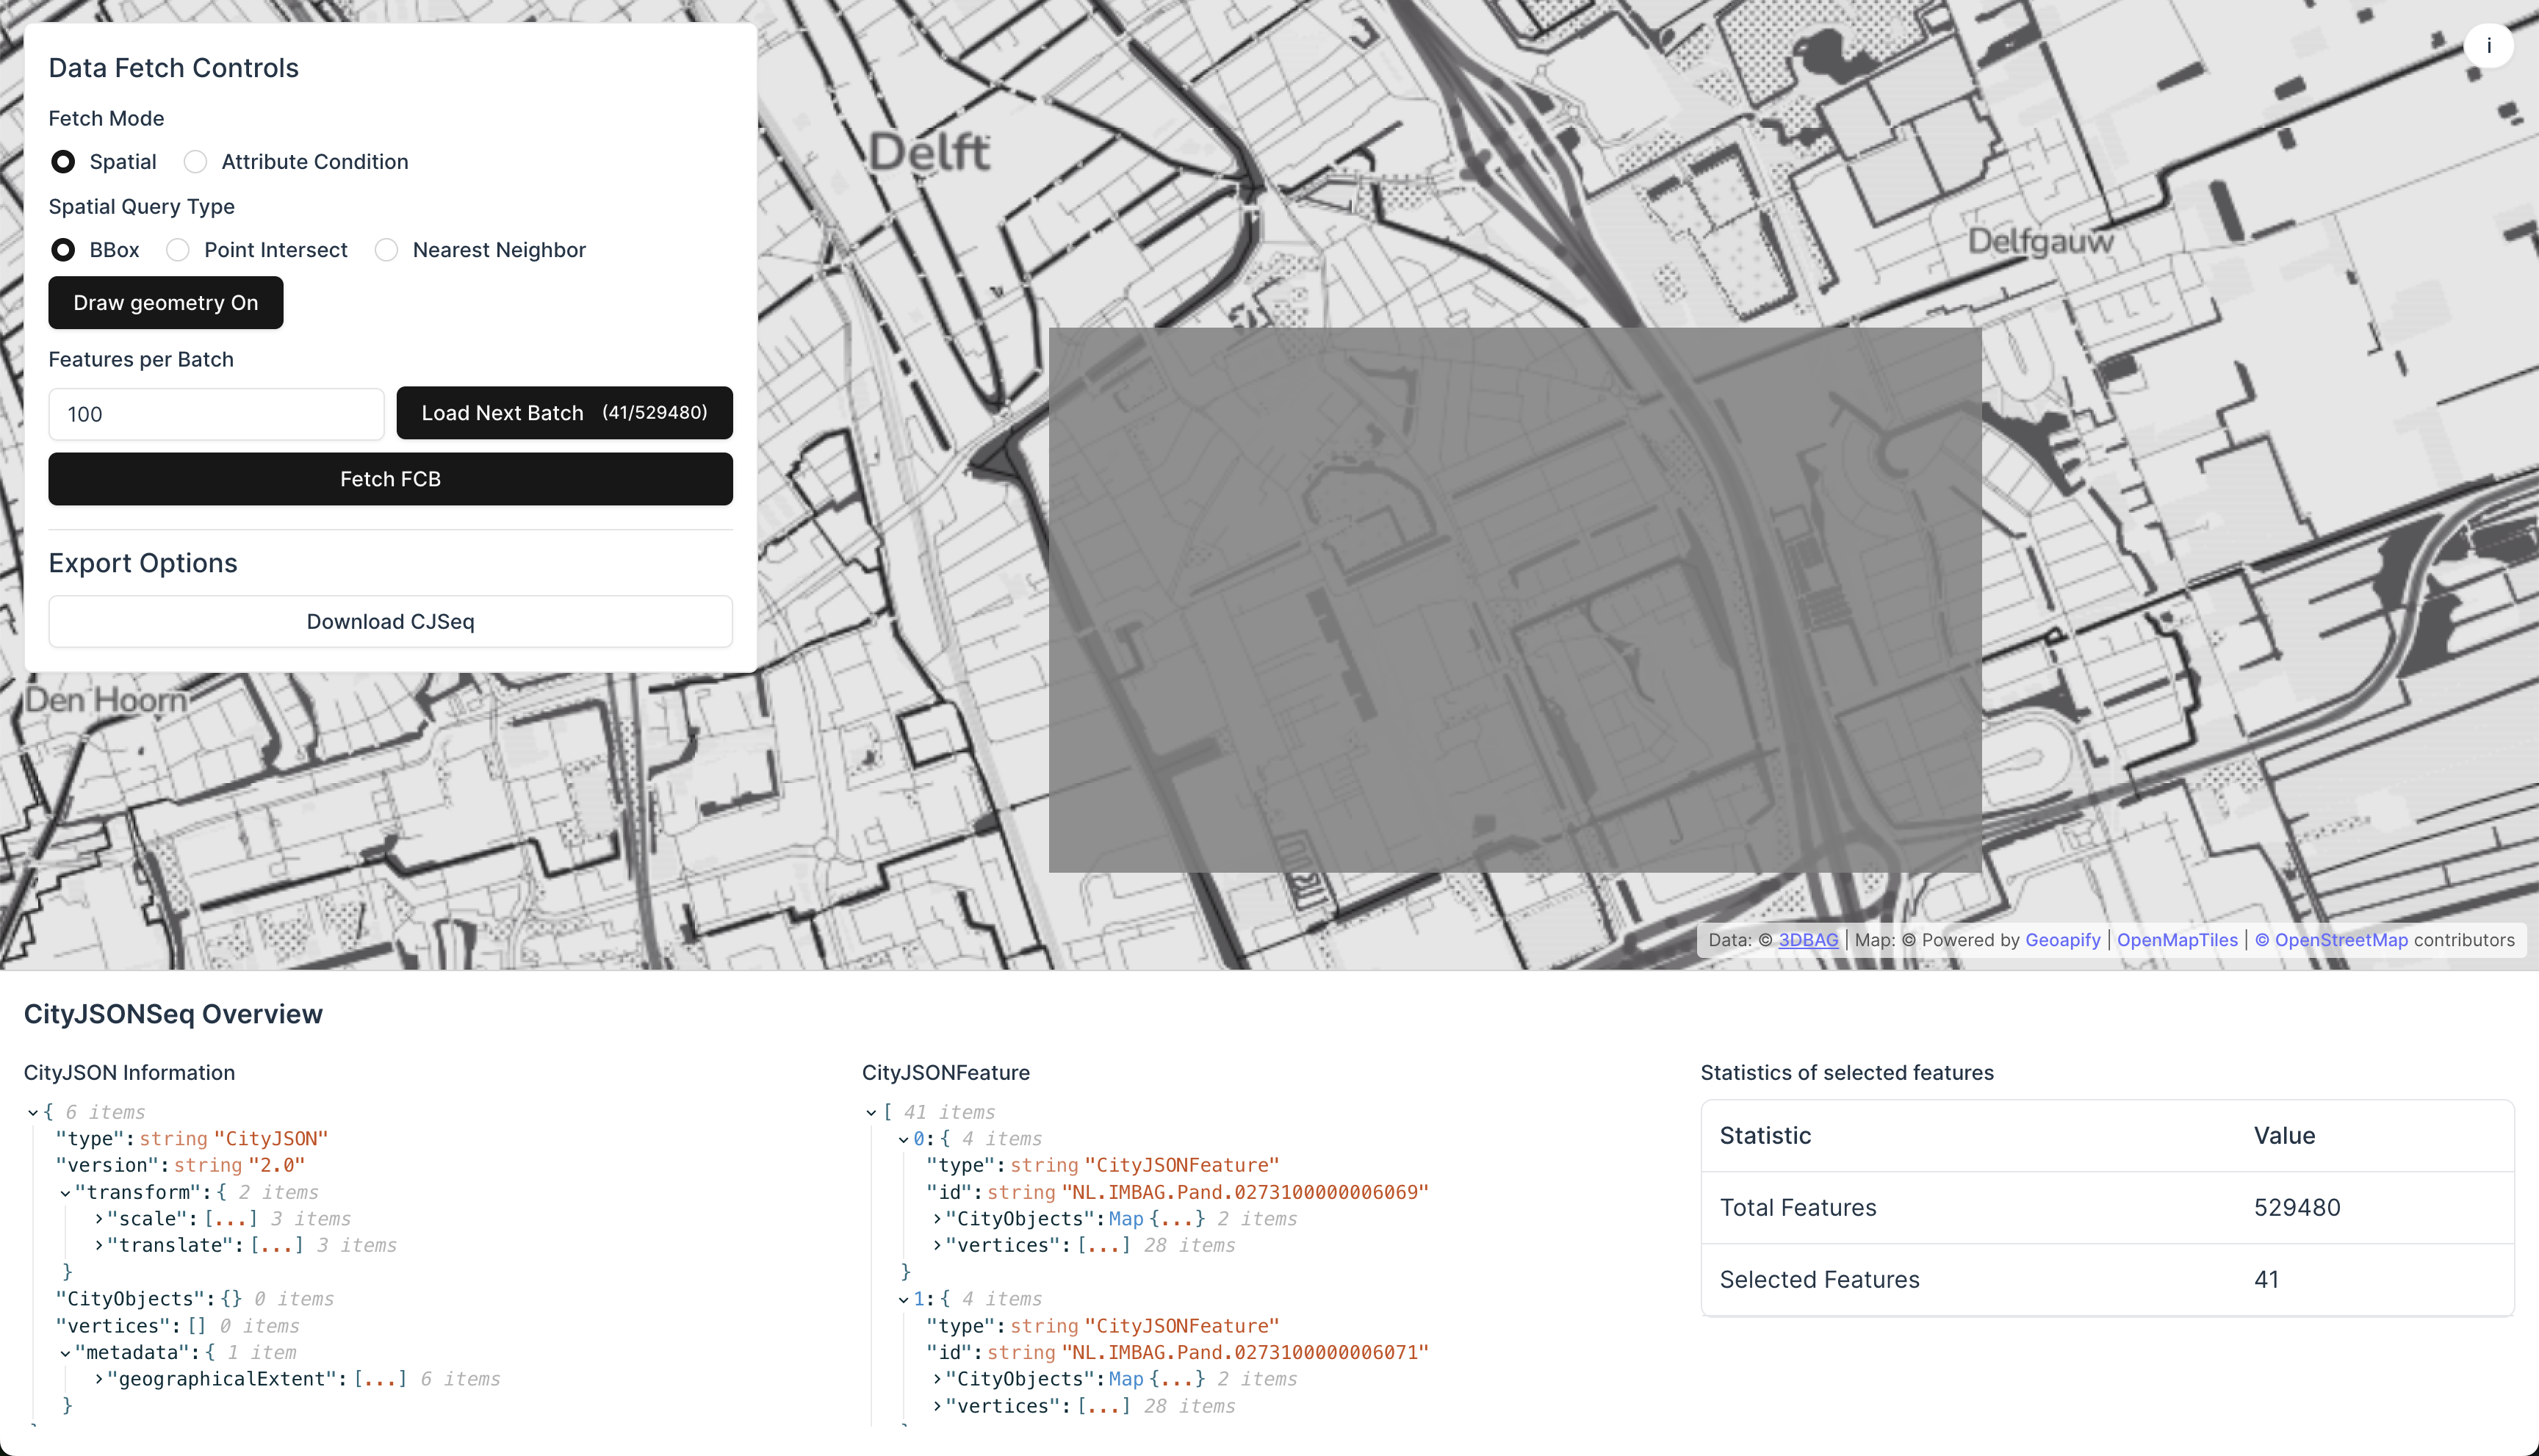
\includegraphics[width=1.0\textwidth]{figs/result_analysis/web_prototype.png}
  \caption{Web prototype of FlatCityBuf demonstrating spatial and attribute query capabilities on a 3.4GB dataset of South Holland.}
  \label{fig:result:cross_platform_implementation:web_prototype}
\end{figure}

\subsection{Integration with Cloud Infrastructure}
\label{result:cross_platform_implementation:cloud_integration}

The HTTP Range Request mechanism integrates seamlessly with modern cloud infrastructure. FlatCityBuf files can be served from standard object storage services like AWS S3, Google Cloud Storage, or Azure Blob Storage, all of which support range requests without additional server-side processing. This enables a serverless architecture where the client-side filtering approach eliminates the need for dedicated server-side processing. This infrastructure compatibility ensures that FlatCityBuf can be deployed in cost-effective cloud environments without requiring specialised application servers and databases.

\begin{figure}[ht]
  \centering
  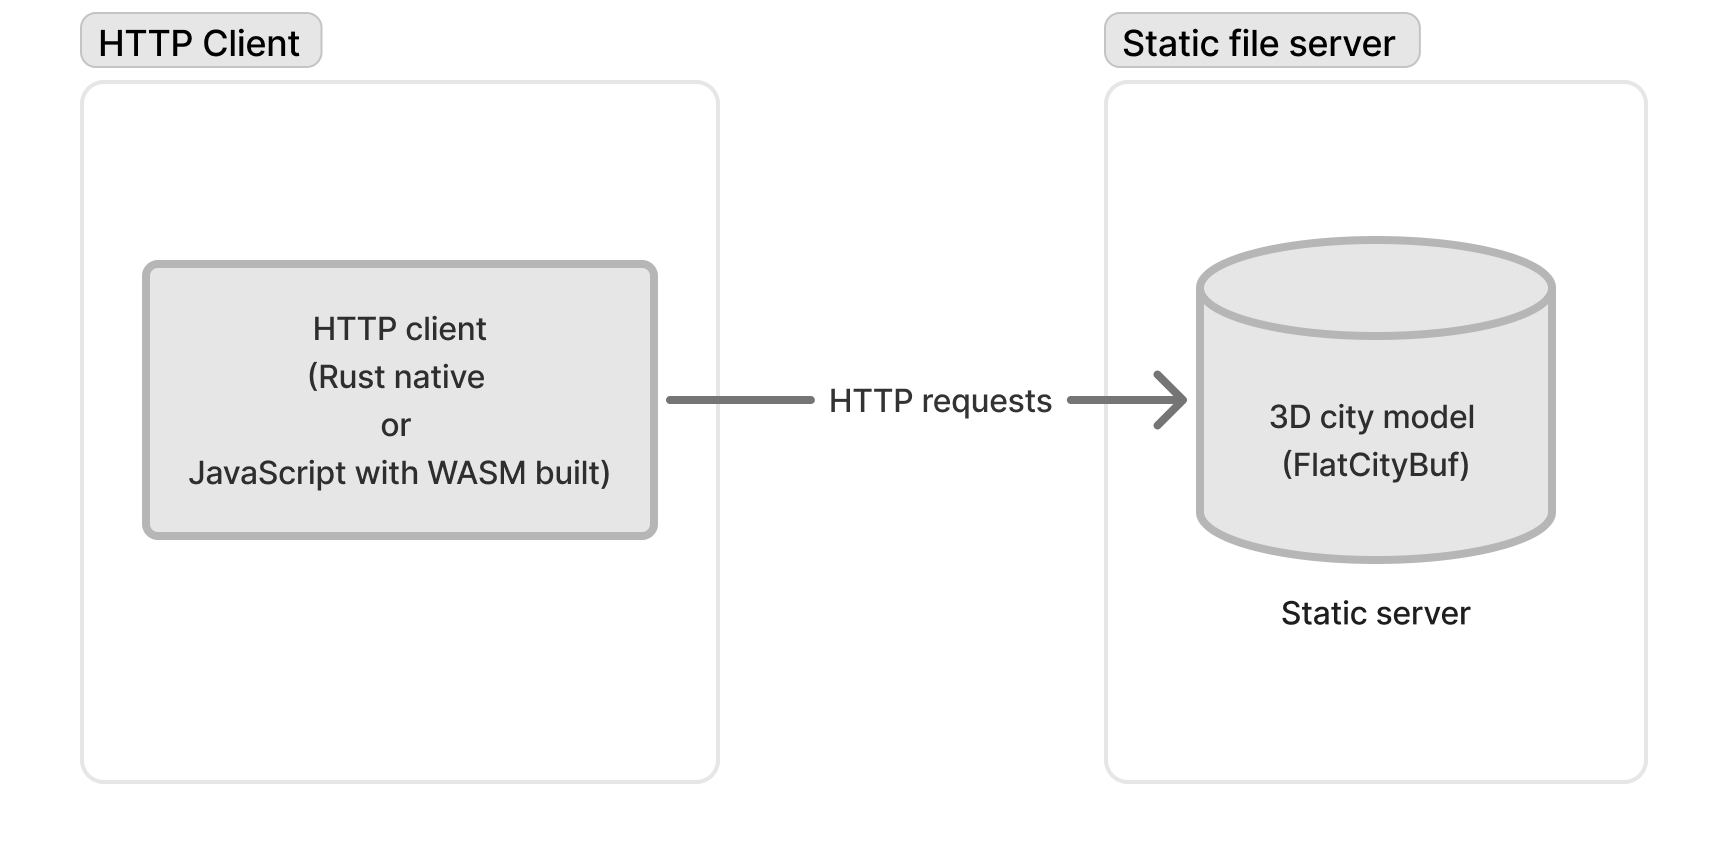
\includegraphics[width=0.8\textwidth]{figs/result_analysis/server_architecture_fcb.png}
  \caption{Server architecture for FlatCityBuf. The client-side filtering approach eliminates the need for dedicated server-side processing.}
  \label{fig:result:cross_platform_implementation:server_architecture}
\end{figure}
\section{Datasets}
\label{result:dataset}

To evaluate file sizes and conduct both local and web-based benchmarks, we employed a diverse range of datasets from \citet{ledoux_2024} supplemented with additional datasets from PLATEAU \citep{plateau}. PLATEAU employs its own data specification combining CityGML 2.0 \citep{CityGML} with a custom \ac{ade}. The CityGML-encoded 3D city models were converted to CityJSON using citygml-tools, a command-line utility developed by \citet{citygml_tools}. Note that PLATEAU's \ac{ade} components are not included in the converted datasets since they are not compatible with the current CityJSON implementation.

To comprehensively evaluate FlatCityBuf, we utilised diverse PLATEAU models including buildings, bridges, transport, tunnels, and vegetation. The dataset collection spans various urban environments from small-scale architectural models to large metropolitan areas across European and Japanese cities, enabling evaluation across different feature types, geometric complexities, and data modeling approaches. \footnote{The datasets used in this evaluation are publicly available at \url{https://github.com/HideBa/flatcitybuf-data}.}

\section{File Size Comparison}
\label{result:file_size_comparison}

\subsection{File size results}
\label{result:overview:filesize_comparison}

\autoref{tab:dataset_comparison} presents a comparison of datasets in both CityJSONSeq and FlatCityBuf formats. The results demonstrate that FlatCityBuf encoding achieves superior compression for several datasets, including Helsinki, Ingolstadt, and New York City, with compression factors of 16.36\%, 19.09\%, and 20.17\% respectively. Conversely, the PLATEAU datasets exhibit the opposite trend, with CityJSONSeq format demonstrating better storage efficiency.
\begin{table*}
  \centering
  \begin{threeparttable}
    \caption{The datasets used for the benchmark.}
    \label{tab:dataset_comparison}
    \scriptsize
    \setlength{\tabcolsep}{1pt}
    \begin{tabular}{@{}lrrlrrr@{\hskip 2pt}rrrr@{}}
      \toprule
      & \multicolumn{3}{c}{\textbf{dataset}} & \multicolumn{3}{c}{\textbf{size of file}} & \multicolumn{4}{c}{\textbf{attributes}} \\
      \cmidrule(lr){2-4} \cmidrule(lr){5-7} \cmidrule(lr){8-11}
      & CityObj & CityFeat & app.$^{\text{(a)}}$ & CityJSONSeq & FlatCityBuf & compr.$^{\text{(b)}}$ & verts & avg$^{\text{(c)}}$ & obj$^{\text{(d)}}$ & sem$^{\text{(e)}}$ \\
      \midrule
      \textbf{3DBAG}          & 2221    & 1110   &      & \qty{5.87}{\mega\byte}  & \qty{6.23}{\mega\byte}  & $-6.02\%$  & 82612    & 74.43    & 37 & 1 \\
      \textbf{3DBV}           & 71634   & 71634  &      & \qty{317.34}{\mega\byte}& \qty{280.92}{\mega\byte}& $11.48\%$  & 4992893  & 69.70    & 64 & 0 \\
      \textbf{Helsinki}       & 77267   & 77231  &      & \qty{412.44}{\mega\byte}& \qty{344.96}{\mega\byte}& $16.36\%$  & 3039107  & 39.35    & 27 & 9 \\
      \textbf{Helsinki\_tex}  & 77267   & 77231  & tex  & \qty{643.70}{\mega\byte}& \qty{545.29}{\mega\byte}& $15.29\%$  & 3039107  & 39.35    & 28 & 9 \\
      \textbf{Ingolstadt}     & 379     & 55     &      & \qty{3.84}{\mega\byte}  & \qty{3.11}{\mega\byte}  & $19.09\%$  & 88001    & 1600.02  & 33 & 13 \\
      \textbf{Montréal}       & 294     & 294    & tex  & \qty{4.60}{\mega\byte}  & \qty{4.80}{\mega\byte}  & $-4.38\%$  & 32242    & 109.67   & 0  & 0 \\
      \textbf{NYC}            & 23777   & 23777  &      & \qty{95.45}{\mega\byte} & \qty{76.20}{\mega\byte} & $20.17\%$  & 1044145  & 43.91    & 3  & 3 \\
      \textbf{Rotterdam}      & 853     & 853    & tex  & \qty{2.69}{\mega\byte}  & \qty{2.80}{\mega\byte}  & $-3.98\%$  & 26679    & 31.28    & 5  & 0 \\
      \textbf{Vienna}         & 1322    & 307    &      & \qty{4.81}{\mega\byte}  & \qty{4.12}{\mega\byte}  & $14.32\%$  & 47229    & 153.84   & 7  & 4 \\
      \textbf{Zürich}         & 198699  & 52834  &      & \qty{247.12}{\mega\byte}& \qty{188.63}{\mega\byte}& $23.67\%$  & 3564542  & 67.47    & 8  & 0 \\
      \textbf{PLATEAU (Building)}  & 10405   & 4307   &      & \qty{76.94}{\mega\byte} & \qty{79.41}{\mega\byte} & $-3.22\%$  & 147754   & 34.31    & 14 & 2 \\
      \textbf{PLATEAU (Bridge)}  & 60      & 8      &      & \qty{4.78}{\mega\byte}  & \qty{5.21}{\mega\byte}  & $-9.09\%$  & 16357    & 2044.62  & 5  & 2 \\
      \textbf{PLATEAU (Railway)}   & 412     & 412    &      & \qty{4.15}{\mega\byte}  & \qty{4.23}{\mega\byte}  & $-1.90\%$  & 5846     & 14.19    & 3  & 2 \\
      \textbf{PLATEAU (Transport)}  & 8136    & 8136   &      & \qty{26.47}{\mega\byte} & \qty{26.62}{\mega\byte} & $-0.54\%$  & 45992    & 5.65     & 3  & 2 \\
      \textbf{PLATEAU (Tunnels)}   & 21      & 3      &      & \qty{4.86}{\mega\byte}  & \qty{4.64}{\mega\byte}  & $4.41\%$   & 12306    & 4102.00  & 4  & 1 \\
      \textbf{PLATEAU (Vegetation)}   & 936     & 936    &      & \qty{1.78}{\mega\byte}  & \qty{2.32}{\mega\byte}  & $-30.50\%$ & 2567     & 2.74     & 3  & 0 \\
      \bottomrule
    \end{tabular}
    \begin{tablenotes}[flushleft]
      \footnotesize
    \item[a] appearance: `tex' indicates textures are stored; `mat' indicates materials are stored
    \item[b] compression factor is $\frac{\text{CityJSONSeq} - \text{FlatCityBuf}}{\text{CityJSONSeq}}$ (positive values indicate size reduction)
    \item[c] average number of vertices per feature
    \item[d] number of attributes in city objects
    \item[e] number of semantic surface attributes in city objects
    \end{tablenotes}
  \end{threeparttable}
\end{table*}

\subsection{Analysis of file size results}
\label{result:overview:analysis_of_file_size_results}
Although \autoref{result:overview:filesize_comparison} provides a summary of file size comparisons, the factors influencing these outcomes require further investigation. This section analyses the underlying causes through controlled experiments with simplified datasets.

\subsubsection{Level of detail}
\label{result:overview:analysis_of_file_size_results:level_of_detail}

To examine how \ac{lod} affects file size, I conducted a series of tests using the TU Delft BK building model at various \ac{lod} levels. Each \ac{lod} variant was systematically extracted from the original model, with attributes and semantic information deliberately removed to isolate the effect of geometric complexity. \autoref{tab:lod_comparison} presents the results of this analysis.

Since each test dataset contains only a single city feature, we compare feature sizes rather than total file sizes. This approach is necessary because FlatCityBuf incorporates a larger header structure, which would disproportionately affect comparisons involving minimal features.

The results demonstrate that while file sizes increase with higher levels of detail, the compression factor remains largely independent of \ac{lod}. Both formats show similar proportional growth in size as geometric complexity increases, with FlatCityBuf consistently achieving approximately 24-25\% size reduction compared to CityJSONSeq regardless of the \ac{lod} level. This suggests that the compression efficiency is determined by the underlying format design rather than the geometric complexity of the data.

\begin{table}[htbp]
  \centering
  \caption{Comparison of file sizes across different levels of detail for the TU Delft BK building model.}
  \label{tab:lod_comparison}
  \begin{tabular}{@{}lrrrr@{}}
    \toprule
    \textbf{Dataset} & \textbf{FlatCityBuf}$^{\text{(a)}}$ & \textbf{CityJSONSeq}$^{\text{(b)}}$ & \textbf{Compression} & \textbf{Vertices} \\
    \midrule
    TUD BK All & \qty{139.75}{\kilo\byte} & \qty{189.01}{\kilo\byte} & $26.08\%$ & 4549 \\
    TUD BK \ac{lod}0 & \qty{12.77}{\kilo\byte} & \qty{20.72}{\kilo\byte} & $38.11\%$ & 785 \\
    TUD BK \ac{lod}1.2 & \qty{37.45}{\kilo\byte} & \qty{49.40}{\kilo\byte} & $24.23\%$ & 1350 \\
    TUD BK \ac{lod}1.3 & \qty{44.66}{\kilo\byte} & \qty{59.25}{\kilo\byte} & $24.67\%$ & 1600 \\
    TUD BK \ac{lod}2.2 & \qty{62.02} {\kilo\byte} & \qty{82.74}{\kilo\byte} & $25.07\%$ & 2168 \\
    \bottomrule
  \end{tabular}
  \begin{tablenotes}[flushleft]
    \footnotesize
  \item[a] Average feature size in bytes in FlatCityBuf: $\frac{\text{Total FlatCityBuf size}}{\text{Number of features}}$
  \item[b] Average feature size in bytes in CityJSONSeq: $\frac{\text{Total CityJSONSeq size}}{\text{Number of features}}$

  \end{tablenotes}
\end{table}

\subsubsection{Attributes}
\label{result:overview:analysis_of_file_size_results:attributes}

To assess the impact of attributes on file size, we tested simple cube models from \citep{cityjson_dataset} with varying numbers of attributes. We systematically generated random attributes for each test case, examining both integer and string data types to determine their effect on compression efficiency. \autoref{tab:attribute_comparison} presents the results of this analysis.

\begin{table}[htbp]
  \centering
  \caption{Comparison of file sizes with varying numbers of attributes for simple cube models.}
  \label{tab:attribute_comparison}
  \begin{tabular}{@{}lrrrr@{}}
    \toprule
    \textbf{Dataset} & \textbf{FlatCityBuf}$^{\text{(a)}}$ & \textbf{CityJSONSeq}$^{\text{(b)}}$ & \textbf{Compression}  \\
    \midrule
    10 attributes (int) & \qty{580}{\byte} & \qty{611}{\byte} & $5.07\%$ \\
    100 attributes (int) & \qty{1.62}{\kilo\byte} & \qty{2.44}{\kilo\byte} & $33.65\%$ \\
    1000 attributes (int) & \qty{12.17}{\kilo\byte} & \qty{21.78}{\kilo\byte} & $44.13\%$ \\
    10 attributes (string) & \qty{580}{\byte} & \qty{611}{\byte} & $5.07\%$ \\
    100 attributes (string) & \qty{1.62}{\kilo\byte} & \qty{2.44}{\kilo\byte} & $33.65\%$ \\
    1000 attributes (string) & \qty{12.17}{\kilo\byte} & \qty{21.78}{\kilo\byte} & $44.13\%$ \\
    \bottomrule
  \end{tabular}
  \begin{tablenotes}[flushleft]
    \footnotesize
  \item[a] Average feature size in bytes in FlatCityBuf: $\frac{\text{Total FlatCityBuf size}}{\text{Number of features}}$
  \item[b] Average feature size in bytes in CityJSONSeq: $\frac{\text{Total CityJSONSeq size}}{\text{Number of features}}$
  \end{tablenotes}
\end{table}

The randomly generated attributes in our test datasets followed a consistent pattern, as shown in the example below:

\begin{lstlisting}[caption={Example of a CityJSON feature with attributes},  basicstyle=\small]
{
  "type": "Building",
  "geometry": [...],
  "attributes": {
    "attr_1": "value_1",
    "attr_2": "value_2",
    "attr_3": "value_3",
    "attr_4": "value_4",
    "attr_5": "value_5",
    ...
    "attr_n": "value_n"
  }
}
\end{lstlisting}

For integer attribute tests, all values were randomly generated integers between 0 and 1000. For string attribute tests, values were randomly generated strings of varying lengths between 5 and 15 characters. This approach ensured a realistic representation of typical attribute data while maintaining controlled test conditions.

\begin{figure}[htbp]
  \centering
  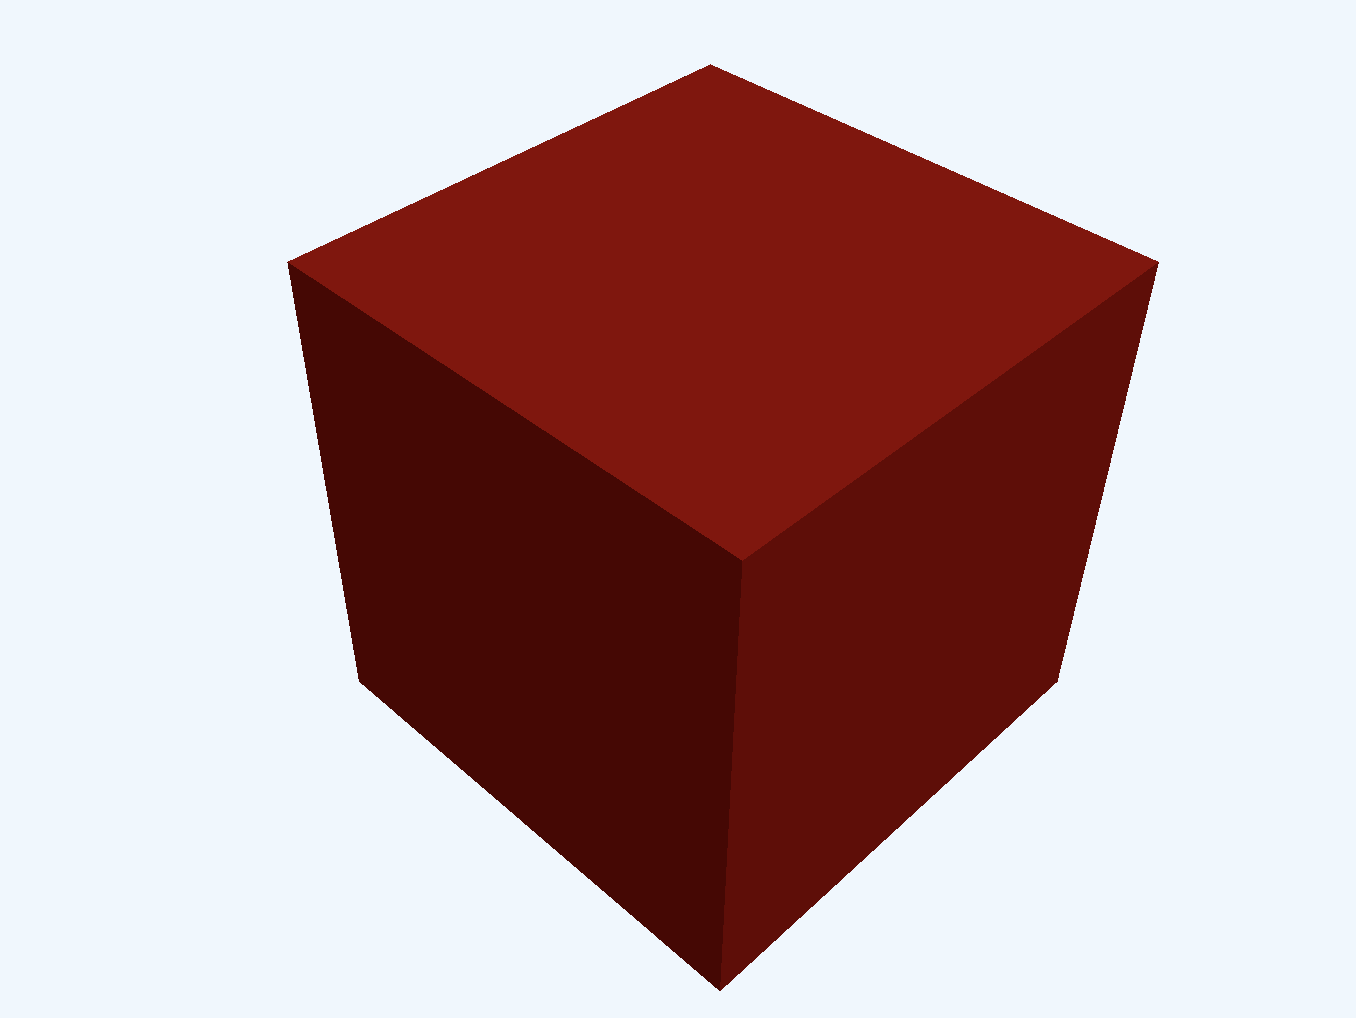
\includegraphics[width=0.48\textwidth]{figs/result_analysis/cube.png}
  \caption{Simple cube model used for attribute testing. This basic geometric structure provides a controlled environment for evaluating the impact of attributes on file size.}
  \label{fig:simple_cube}
\end{figure}

The results reveal a clear pattern: FlatCityBuf's compression advantage over CityJSONSeq increases substantially with the number of attributes. With only 10 attributes, the compression benefit is minimal at 5.07\%, but rises markedly to 33.65\% with 100 attributes and reaches 44.13\% with 1000 attributes.

This efficiency stems from FlatCityBuf's architectural design, which stores the attribute schema once in the file header. Each feature subsequently references attributes using only a 2-byte (u16) index, while CityJSONSeq must replicate identical attribute keys across all features. Although additional attributes increase the header size, this overhead is distributed across all features in the dataset. The header remains relatively compact—even with 1000 attributes, it occupies only a few tens of kilobytes.

These characteristics render FlatCityBuf particularly advantageous for datasets containing numerous attributes. The same efficiency applies to semantic surface attributes, where the schema-based approach provides similar compression benefits when features contain multiple surfaces with rich semantic information.

\subsubsection{Geometry complexity}
\label{result:overview:analysis_of_file_size_results:geometric_complexity}

To evaluate how geometric complexity influences file size, we analysed models with varying numbers of vertices. The test utilised two geometrically distinct models from the TU Delft campus dataset—one simple and one complex. To isolate the effect of geometry, attributes and semantic information were removed, leaving only the essential geometric components required by CityJSON. \autoref{tab:geometry_comparison} presents the numerical results of this analysis, while \autoref{fig:geometry_comparison} provides visual comparisons of the models.

\begin{table}[htbp]
  \centering
  \caption{Comparison of file sizes with varying geometric complexity.}
  \label{tab:geometry_comparison}
  \begin{tabular}{@{}lrrrr@{}}
    \toprule
    \textbf{Dataset} & \textbf{FlatCityBuf}$^{\text{(a)}}$ & \textbf{CityJSONSeq}$^{\text{(b)}}$ & \textbf{Compression} & \textbf{Vertices/Feature} \\
    \midrule
    TUD BK & \qty{139.75}{\kilo\byte} & \qty{189.01}{\kilo\byte} & $26.06\%$ & 4549 \\
    TUD Simple & \qty{13.12}{\kilo\byte} & \qty{15.42}{\kilo\byte} & $14.94\%$ & 340 \\
    \bottomrule
  \end{tabular}
  \begin{tablenotes}[flushleft]
    \footnotesize
  \item[a] Average feature size in bytes in FlatCityBuf: $\frac{\text{Total FlatCityBuf size}}{\text{Number of features}}$
  \item[b] Average feature size in bytes in CityJSONSeq: $\frac{\text{Total CityJSONSeq size}}{\text{Number of features}}$
  \end{tablenotes}
\end{table}

\begin{figure}[htbp]
  \centering
  \begin{subfigure}{0.48\textwidth}
    \centering
    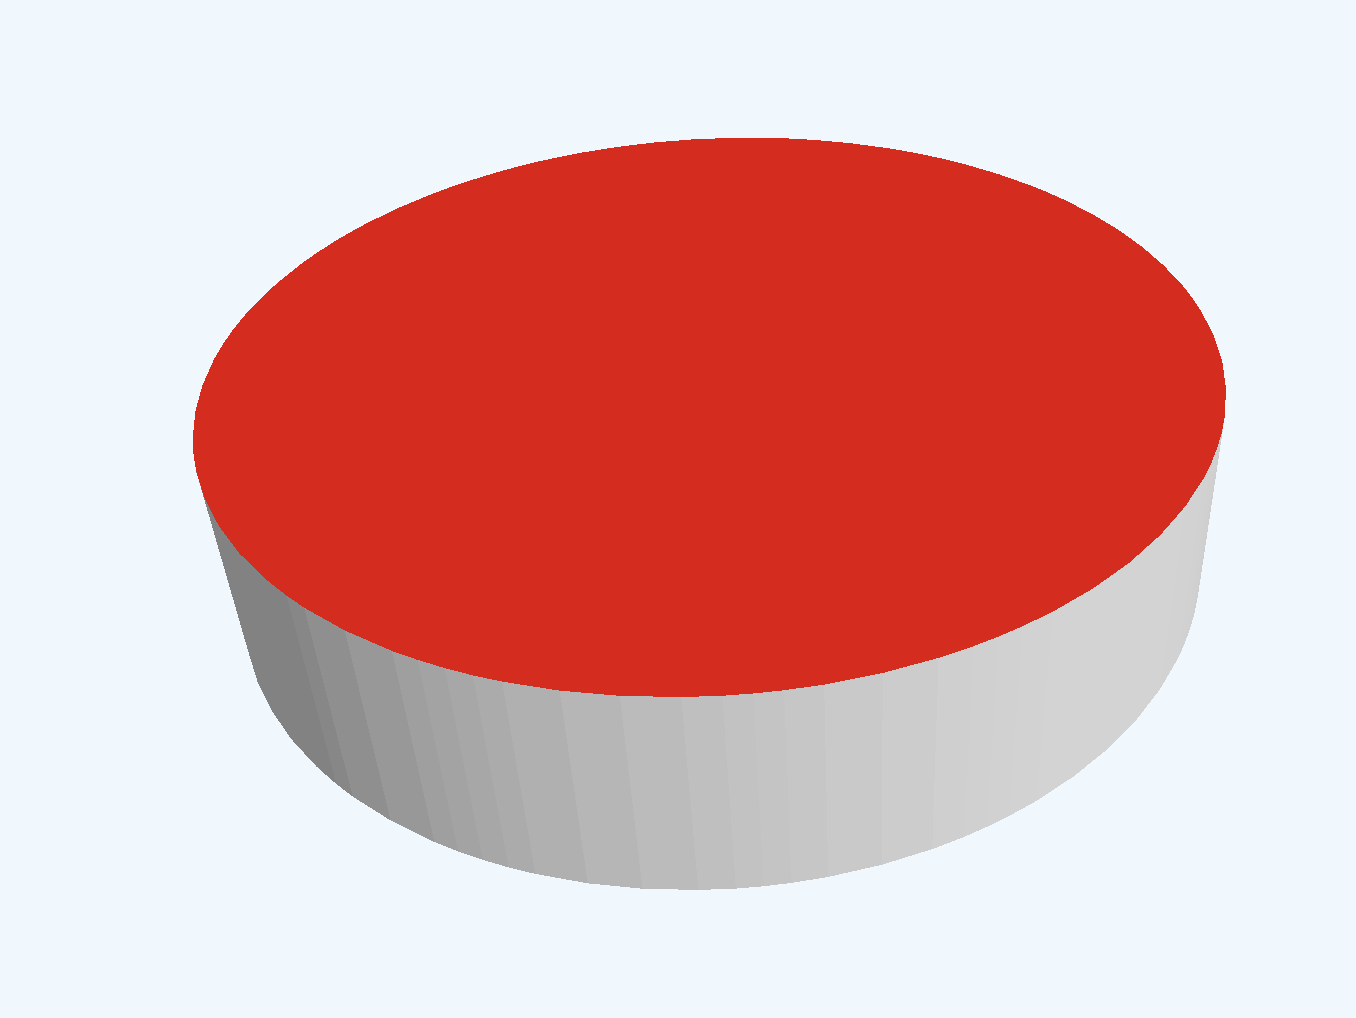
\includegraphics[width=\textwidth]{figs/result_analysis/tud_simple.png}
    \caption{TUD Simple model (340 vertices/feature)}
    \label{fig:tud_simple}
  \end{subfigure}
  \hfill
  \begin{subfigure}{0.48\textwidth}
    \centering
    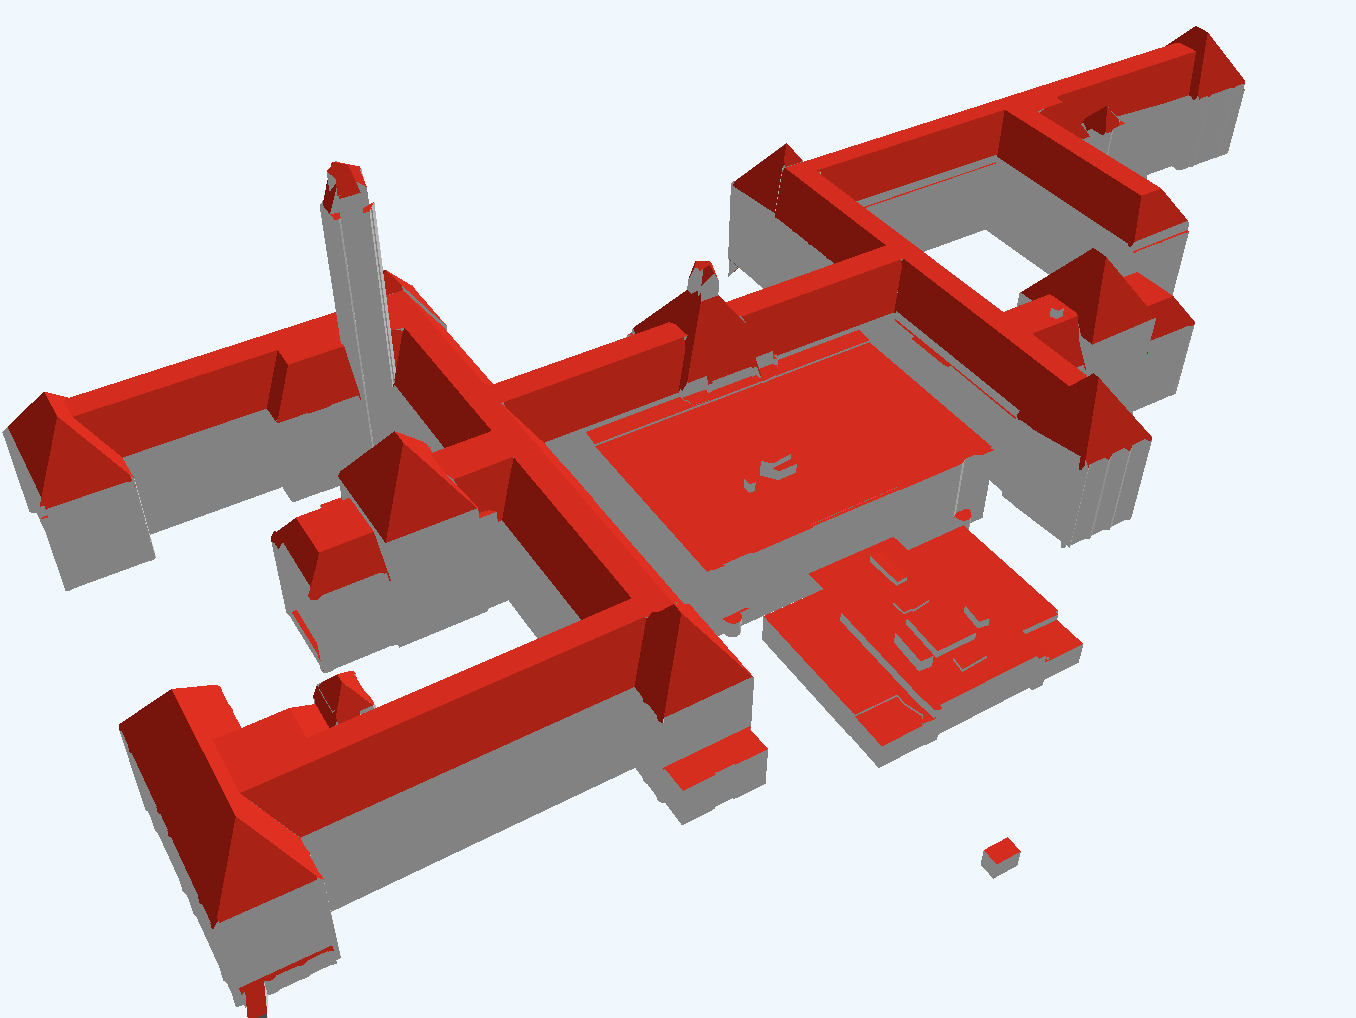
\includegraphics[width=\textwidth]{figs/result_analysis/tud_bk.png}
    \caption{TUD BK model (4549 vertices/feature)}
    \label{fig:tud_bk}
  \end{subfigure}
  \caption{Visual comparison of models with different geometric complexity.}
  \label{fig:geometry_comparison}
\end{figure}

The results demonstrate that geometric complexity significantly affects compression efficiency, with FlatCityBuf achieving better compression for more intricate models. The TU Delft BK building model, containing 4549 vertices per feature, exhibits a higher compression rate of 26.06\% compared to the simpler model with 340 vertices at 14.94\%.

This differential appears to result from the expanding boundary field as geometry becomes more complex. FlatCityBuf employs a strongly typed representation of boundaries (using u32 integers) that maintains a constant size for encoding each vertex, whereas CityJSONSeq requires additional bytes due to its text-based format. This fundamental difference in geometry encoding becomes increasingly advantageous for FlatCityBuf as geometric complexity rises.

\subsubsection{Vertices and coordinates}
\label{result:overview:analysis_of_file_size_results:vertices_and_coordinates}

To investigate how coordinate scale affects file size, I conducted tests using identical cube geometries with different coordinate magnitudes. All test models represent the same simple cube shape with identical geometric complexity (8 vertices per feature), but the coordinate values are scaled to different magnitudes—ranging from single digits to millions—while maintaining the same spatial relationships. \autoref{tab:vertices_comparison} presents the results of this analysis, utilising the same base cube geometry as in \autoref{result:overview:analysis_of_file_size_results:attributes}.

\begin{table}[htbp]
  \centering
  \caption{Comparison of file sizes with varying coordinate scales.}
  \label{tab:vertices_comparison}
  \begin{tabular}{@{}lrrrr@{}}
    \toprule
    \textbf{Dataset} & \textbf{FlatCityBuf}$^{\text{(a)}}$ & \textbf{CityJSONSeq}$^{\text{(b)}}$ & \textbf{Compression} & \textbf{Scale} \\
    \midrule
    Cube (1) & \qty{476}{\byte} & \qty{370}{\byte} & $-28.65\%$ & 1 \\
    Cube (10) & \qty{476}{\byte} & \qty{459}{\byte} & $-3.70\%$ & 10 \\
    Cube (1k) & \qty{476}{\byte} & \qty{507}{\byte} & $6.11\%$ & 1,000 \\
    Cube (1M) & \qty{476}{\byte} & \qty{579}{\byte} & $17.79\%$ & 1,000,000 \\
    \bottomrule
  \end{tabular}
  \begin{tablenotes}[flushleft]
    \footnotesize
  \item[a] Average feature size in bytes in FlatCityBuf: $\frac{\text{Total FlatCityBuf size}}{\text{Number of features}}$
  \item[b] Average feature size in bytes in CityJSONSeq: $\frac{\text{Total CityJSONSeq size}}{\text{Number of features}}$
  \end{tablenotes}
\end{table}

The results reveal an intriguing relationship between coordinate scale and file size in both formats. FlatCityBuf maintains a consistent size of 476 bytes regardless of coordinate magnitude, demonstrating its fixed-size binary encoding for numeric values. In contrast, CityJSONSeq's file size increases proportionally with larger coordinate values, growing from 370 bytes with single-digit coordinates to 579 bytes with million-scale coordinates.

This behaviour occurs because both FlatCityBuf and CityJSONSeq use integer values as coordinates, which are quantised by the \texttt{Transform} field as explained in \autoref{rw:cityjson:coordinate_quantisation}. However, FlatCityBuf stores these coordinates as fixed-size 32-bit integers, while CityJSONSeq, being a text-based format, requires more characters to represent larger numbers. Consequently, FlatCityBuf transitions from being less efficient than CityJSONSeq for small coordinate values (-28.65\%) to substantially more efficient for large coordinate values (17.79\%).

This characteristic explains the pattern observed in \autoref{result:overview:filesize_comparison}. FlatCityBuf demonstrates lower storage efficiency for PLATEAU datasets, likely because these datasets employ geographic coordinate systems with values typically between -180 and 180. Since CityJSON quantises coordinates through the \texttt{Transform} field, latitude and longitude values can be represented as relatively small integers. Conversely, datasets where FlatCityBuf performs better—such as NYC and Helsinki—use local coordinate systems (in metres) with larger internal values, resulting in improved compression efficiency with FlatCityBuf.

\subsubsection{Summary of File Size Analysis}
\label{result:overview:analysis_of_file_size_results:summary}

The comprehensive analysis of various factors affecting file size reveals distinct patterns in the compression performance of FlatCityBuf compared to CityJSONSeq:

\begin{itemize}
  \item \textbf{Level of Detail:} The analysis demonstrates that geometric detail levels have minimal impact on compression efficiency. While file sizes naturally increase with higher \ac{lod}s, the compression advantage of FlatCityBuf remains relatively consistent at approximately 24-25\% across different levels of geometric complexity.

  \item \textbf{Attribute Quantity:} The number of attributes significantly influences compression performance. FlatCityBuf's efficiency increases dramatically with attribute count, from minimal compression (5.07\%) with 10 attributes to substantial compression (44.13\%) with 1000 attributes. This progressive advantage stems from FlatCityBuf's schema-based approach that eliminates redundant attribute key storage.

  \item \textbf{Geometric Complexity:} More intricate geometries benefit from improved compression with FlatCityBuf. As boundary fields expand with geometric complexity, FlatCityBuf's fixed-size numeric representation provides greater efficiency compared to the text-based encoding of CityJSONSeq, increasing compression from 14.94\% for simple geometries to 26.06\% for complex models.

  \item \textbf{Coordinate Scale:} The magnitude of coordinate values has a significant impact on compression efficiency. FlatCityBuf's constant-size integer representation maintains consistent file sizes regardless of coordinate scale, while CityJSONSeq requires more space for larger values. This creates a transition from inferior compression (-28.65\%) with small coordinate values to superior compression (17.79\%) with large coordinate values.
\end{itemize}

These findings elucidate the observed variations in compression performance across different datasets in \autoref{tab:dataset_comparison}. FlatCityBuf demonstrates optimal performance for datasets with numerous attributes, complex geometries, and large-scale coordinate systems, while CityJSONSeq may retain advantages for simpler datasets with limited attributes and smaller coordinate values.

\section{Benchmark on Local Environment}
\label{result:benchmark_on_local_environment}

This section presents a comprehensive performance evaluation of the FlatCityBuf format conducted in a controlled local environment. The analysis focuses on critical metrics including read operations, memory utilisation, and processing efficiency to establish a thorough understanding of the format's performance characteristics.

\subsection{Test Environment}
\label{result:benchmark_on_local_environment:test_environment}

All benchmarks were executed within a consistent hardware and software configuration to ensure reliability and reproducibility:

\begin{itemize}
  \item \textbf{Hardware:} Apple MacBook Pro with M1 Max chip, 32GB unified memory
  \item \textbf{Operating System:} macOS Sequoia 15.4
  \item \textbf{Storage:} 1TB SSD with approximately 200GB available capacity
  \item \textbf{Runtime Environment:} Rust 1.86.0, with optimised release builds
\end{itemize}

\subsection{Measurement Parameters}
\label{result:benchmark_on_local_environment:measurement_parameters}

The benchmark framework captured multiple performance dimensions through the following key indicators:
\todo{Ravi's comment "you could also look at write performance here"}

\begin{itemize}
  \item \textbf{Read Performance:} Time required to deserialise the file and map the data into memory using zero-copy techniques, measured in milliseconds with microsecond precision

  \item \textbf{Memory Efficiency:} Peak Resident Set Size (RSS) during file processing, providing an accurate measurement of maximum memory requirements

\end{itemize}
These parameters were systematically measured across all encoding formats—CityJSONSeq, CBOR, BSON, and FlatCityBuf—to facilitate direct performance comparisons. CBOR and BSON were selected as additional comparison formats because they are JSON-compatible binary encoding formats, providing a meaningful intermediate comparison between text-based CityJSONSeq and the custom FlatCityBuf implementation. For CBOR and BSON evaluation, single CityJSON files were encoded, which serve as the source for the corresponding CityJSONSeq datasets. Other data formats such as Protocol Buffers or GeoParquet would require developing dedicated libraries similar to the FlatBuffers implementation, making them less suitable for this comparative analysis. The subsequent sections present a detailed analysis of these measurements and their implications for practical applications.

\subsection{Read Performance FlatCityBuf vs CityJSONSeq}
\label{result:benchmark_on_local_environment:read_performance_flatcitybuf_vs_cityjsonseq}

The performance comparison between FlatCityBuf and CityJSONSeq was conducted across multiple datasets, measuring processing time, and memory consumption as key metrics. \autoref{tab:performance_comparison} presents these results.

\begin{table}[ht]
  \centering
  \begin{threeparttable}
    \caption{Performance comparison between CityJSONSeq and FlatCityBuf}
    \label{tab:performance_comparison}
    \setlength{\tabcolsep}{10pt}
    \scriptsize
    \begin{tabular}{@{}l|rrr|rrr@{}}
      \toprule
      & \multicolumn{3}{c|}{\textbf{Processing Time}}
      & \multicolumn{3}{c}{\textbf{Memory Consumption}} \\
      \cmidrule(lr){2-4} \cmidrule(lr){5-7}
      \textbf{Dataset}
      & \textbf{cjseq\tnote{a}} & \textbf{FlatCityBuf} & \textbf{Ratio\tnote{b}}
      & \textbf{cjseq\tnote{a}} & \textbf{FlatCityBuf} & \textbf{Ratio\tnote{b}} \\
      \midrule
      3DBAG
      & \qty{56.3}{\milli\second} & \qty{6.6}{\milli\second} & 8.6$\times$
      & \qty{23.9}{\mega\byte} & \qty{5.1}{\mega\byte} & 4.7$\times$ \\

      3DBV
      & \qty{3.99}{\second} & \qty{122.5}{\milli\second} & 32.6$\times$
      & \qty{283.8}{\mega\byte} & \qty{63.2}{\mega\byte} & 4.5$\times$ \\

      Helsinki
      & \qty{4.05}{\second} & \qty{132.2}{\milli\second} & 30.6$\times$
      & \qty{15.3}{\mega\byte} & \qty{5.2}{\mega\byte} & 2.9$\times$ \\

      Ingolstadt
      & \qty{37.2}{\milli\second} & \qty{0.5}{\milli\second} & 75.8$\times$
      & \qty{30.1}{\mega\byte} & \qty{6.9}{\mega\byte} & 4.4$\times$ \\

      Montréal
      & \qty{50.3}{\milli\second} & \qty{0.6}{\milli\second} & 81.6$\times$
      & \qty{36.3}{\mega\byte} & \qty{5.7}{\mega\byte} & 6.4$\times$ \\

      NYC
      & \qty{887.6}{\milli\second} & \qty{42.9}{\milli\second} & 20.7$\times$
      & \qty{20.6}{\mega\byte} & \qty{5.0}{\mega\byte} & 4.1$\times$ \\

      Rotterdam
      & \qty{22.2}{\milli\second} & \qty{1.3}{\milli\second} & 17.6$\times$
      & \qty{9.2}{\mega\byte} & \qty{4.4}{\mega\byte} & 2.1$\times$ \\

      Vienna
      & \qty{45.9}{\milli\second} & \qty{1.9}{\milli\second} & 24.0$\times$
      & \qty{14.6}{\mega\byte} & \qty{5.2}{\mega\byte} & 2.8$\times$ \\

      Zürich
      & \qty{1.88}{\second} & \qty{151.9}{\milli\second} & 12.4$\times$
      & \qty{31.3}{\mega\byte} & \qty{5.1}{\mega\byte} & 6.2$\times$ \\

      PLATEAU (Building)
      & \qty{861.4}{\milli\second} & \qty{32.5}{\milli\second} & 26.5$\times$
      & \qty{220.9}{\mega\byte} & \qty{64.4}{\mega\byte} & 3.4$\times$ \\

      PLATEAU (Bridge)
      & \qty{83.9}{\milli\second} & \qty{0.3}{\milli\second} & 256.8$\times$
      & \qty{75.0}{\mega\byte} & \qty{12.0}{\mega\byte} & 6.3$\times$ \\

      PLATEAU (Railway)
      & \qty{37.9}{\milli\second} & \qty{2.0}{\milli\second} & 18.5$\times$
      & \qty{19.0}{\mega\byte} & \qty{5.1}{\mega\byte} & 3.8$\times$ \\

      PLATEAU (Transport)
      & \qty{244.0}{\milli\second} & \qty{13.3}{\milli\second} & 18.4$\times$
      & \qty{76.7}{\mega\byte} & \qty{20.2}{\mega\byte} & 3.8$\times$ \\

      PLATEAU (Tunnels)
      & \qty{47.9}{\milli\second} & \qty{1.9}{\milli\second} & 24.9$\times$
      & \qty{70.6}{\mega\byte} & \qty{12.6}{\mega\byte} & 5.6$\times$ \\

      PLATEAU (Vegetation)
      & \qty{852.3}{\milli\second} & \qty{32.9}{\milli\second} & 25.9$\times$
      & \qty{189.8}{\mega\byte} & \qty{56.9}{\mega\byte} & 3.3$\times$ \\

      \bottomrule
    \end{tabular}
    \begin{tablenotes}[flushleft]
      \footnotesize
    \item[a] CityJSONSeq
    \item[b] Ratio = CityJSONSeq metric / FlatCityBuf metric (higher values indicate better FlatCityBuf performance)
    \end{tablenotes}
  \end{threeparttable}
\end{table}

The performance comparison reveals significant advantages for FlatCityBuf in both processing time and memory consumption. FlatCityBuf demonstrates consistently superior performance, processing data between 8.6$\times$ and 256.8$\times$ faster than CityJSONSeq across all datasets. The most dramatic improvements are observed for the PLATEAU bridge model and Ingolstadt datasets, which suggests that FlatCityBuf exhibits lower overhead when handling smaller datasets. Memory consumption is also consistently reduced compared to CityJSONSeq, with FlatCityBuf showing particularly notable advantages for certain datasets, including Montréal and the PLATEAU Bridge model.

\subsection{Read performance FlatCityBuf vs CBOR}
\label{result:benchmark_on_local_environment:read_performance_flatcitybuf_vs_cbor}

The performance comparison between FlatCityBuf and CBOR was conducted using the same datasets and measurement methodology. \autoref{tab:performance_comparison_cbor} presents these results.

\begin{table}[ht]
  \centering
  \begin{threeparttable}
    \caption{Performance comparison between CBOR and FlatCityBuf}
    \label{tab:performance_comparison_cbor}
    \setlength{\tabcolsep}{10pt}
    \scriptsize
    \begin{tabular}{@{}l|rrr|rrr@{}}
      \toprule
      & \multicolumn{3}{c|}{\textbf{Processing Time}}
      & \multicolumn{3}{c}{\textbf{Memory Consumption}} \\
      \cmidrule(lr){2-4} \cmidrule(lr){5-7}
      \textbf{Dataset}
      & \textbf{CBOR} & \textbf{FlatCityBuf} & \textbf{Ratio\tnote{a}}
      & \textbf{CBOR} & \textbf{FlatCityBuf} & \textbf{Ratio\tnote{a}} \\
      \midrule
      3DBAG
      & \qty{74.0}{\milli\second} & \qty{6.6}{\milli\second} & 11.2$\times$
      & \qty{194.1}{\mega\byte} & \qty{5.1}{\mega\byte} & 38.1$\times$ \\

      3DBV
      & \qty{6.34}{\second} & \qty{122.5}{\milli\second} & 51.8$\times$
      & \qty{4.96}{\giga\byte} & \qty{63.2}{\mega\byte} & 80.3$\times$ \\

      Helsinki
      & \qty{7.97}{\second} & \qty{132.2}{\milli\second} & 60.3$\times$
      & \qty{5.14}{\giga\byte} & \qty{5.2}{\mega\byte} & 1011.2$\times$ \\

      Ingolstadt
      & \qty{46.9}{\milli\second} & \qty{0.5}{\milli\second} & 95.7$\times$
      & \qty{187.5}{\mega\byte} & \qty{6.9}{\mega\byte} & 27.3$\times$ \\

      Montréal
      & \qty{58.4}{\milli\second} & \qty{0.6}{\milli\second} & 94.7$\times$
      & \qty{257.1}{\mega\byte} & \qty{5.7}{\mega\byte} & 45.3$\times$ \\

      NYC
      & \qty{1.33}{\second} & \qty{42.9}{\milli\second} & 31.0$\times$
      & \qty{1.65}{\giga\byte} & \qty{5.0}{\mega\byte} & 337.4$\times$ \\

      Rotterdam
      & \qty{30.8}{\milli\second} & \qty{1.3}{\milli\second} & 24.4$\times$
      & \qty{140.0}{\mega\byte} & \qty{4.4}{\mega\byte} & 31.9$\times$ \\

      Vienna
      & \qty{58.8}{\milli\second} & \qty{1.9}{\milli\second} & 30.7$\times$
      & \qty{179.8}{\mega\byte} & \qty{5.2}{\mega\byte} & 34.7$\times$ \\

      Zürich
      & \qty{3.53}{\second} & \qty{151.9}{\milli\second} & 23.3$\times$
      & \qty{4.51}{\giga\byte} & \qty{5.1}{\mega\byte} & 913.2$\times$ \\

      PLATEAU (Building)
      & \qty{1.06}{\second} & \qty{32.5}{\milli\second} & 32.4$\times$
      & \qty{1.83}{\giga\byte} & \qty{64.4}{\mega\byte} & 28.4$\times$ \\

      PLATEAU (Bridge)
      & \qty{63.6}{\milli\second} & \qty{0.3}{\milli\second} & 194.7$\times$
      & \qty{305.4}{\mega\byte} & \qty{12.0}{\mega\byte} & 25.6$\times$ \\

      PLATEAU (Railway)
      & \qty{46.3}{\milli\second} & \qty{2.0}{\milli\second} & 22.7$\times$
      & \qty{141.0}{\mega\byte} & \qty{5.1}{\mega\byte} & 27.9$\times$ \\

      PLATEAU (Transport)
      & \qty{316.1}{\milli\second} & \qty{13.3}{\milli\second} & 23.8$\times$
      & \qty{614.5}{\mega\byte} & \qty{20.2}{\mega\byte} & 30.5$\times$ \\

      PLATEAU (Tunnels)
      & \qty{147.7}{\milli\second} & \qty{1.9}{\milli\second} & 76.7$\times$
      & \qty{400.2}{\mega\byte} & \qty{12.6}{\mega\byte} & 31.8$\times$ \\

      PLATEAU (Vegetation)
      & \qty{997.8}{\milli\second} & \qty{32.9}{\milli\second} & 30.3$\times$
      & \qty{1.97}{\giga\byte} & \qty{56.9}{\mega\byte} & 35.3$\times$ \\

      \bottomrule
    \end{tabular}
    \begin{tablenotes}[flushleft]
      \footnotesize
    \item[a] Ratio = CBOR metric / FlatCityBuf metric (higher values indicate better FlatCityBuf performance)
    \end{tablenotes}
  \end{threeparttable}
\end{table}

The benchmark results demonstrate that FlatCityBuf consistently outperforms CBOR across all tested datasets. When compared to CBOR, FlatCityBuf achieved processing time improvements ranging from 11.2$\times$ to 194.7$\times$, with particularly significant speedups observed for smaller datasets such as the PLATEAU bridge model and Ingolstadt. This pattern reflects FlatCityBuf's zero-copy deserialization advantage, which provides proportionally greater benefits when parsing overhead dominates the total processing time in smaller datasets.

Memory consumption was reduced by factors ranging from 25.6$\times$ to 1011.2$\times$, with the most dramatic improvements observed in larger datasets such as Helsinki and Zürich. This trend occurs because CBOR requires loading the entire dataset into memory during deserialization, while FlatCityBuf's zero-copy approach allows selective access without full memory allocation. As dataset size increases, this fundamental difference in memory management strategy becomes increasingly pronounced.

\subsection{Read performance FlatCityBuf vs BSON}
\label{result:benchmark_on_local_environment:read_performance_flatcitybuf_vs_bson}

The performance comparison between FlatCityBuf and BSON followed the same methodology as the previous comparisons. \autoref{tab:performance_comparison_bson} presents the detailed results.

\begin{table}[ht]
  \centering
  \begin{threeparttable}
    \caption{Performance comparison between BSON and FlatCityBuf}
    \label{tab:performance_comparison_bson}
    \setlength{\tabcolsep}{10pt}
    \scriptsize
    \begin{tabular}{@{}l|rrr|rrr@{}}
      \toprule
      & \multicolumn{3}{c|}{\textbf{Processing Time}}
      & \multicolumn{3}{c}{\textbf{Memory Consumption}} \\
      \cmidrule(lr){2-4} \cmidrule(lr){5-7}
      \textbf{Dataset}
      & \textbf{BSON} & \textbf{FlatCityBuf} & \textbf{Ratio\tnote{a}}
      & \textbf{BSON} & \textbf{FlatCityBuf} & \textbf{Ratio\tnote{a}} \\
      \midrule
      3DBAG
      & \qty{117.1}{\milli\second} & \qty{6.6}{\milli\second} & 17.8$\times$
      & \qty{276.8}{\mega\byte} & \qty{5.1}{\mega\byte} & 54.3$\times$ \\

      3DBV
      & \qty{9.97}{\second} & \qty{122.5}{\milli\second} & 81.4$\times$
      & \qty{6.38}{\giga\byte} & \qty{63.2}{\mega\byte} & 103.4$\times$ \\

      Helsinki
      & \qty{14.64}{\second} & \qty{132.2}{\milli\second} & 110.7$\times$
      & \qty{6.77}{\giga\byte} & \qty{5.2}{\mega\byte} & 1331.7$\times$ \\

      Ingolstadt
      & \qty{79.9}{\milli\second} & \qty{0.5}{\milli\second} & 163.1$\times$
      & \qty{267.3}{\mega\byte} & \qty{6.9}{\mega\byte} & 38.9$\times$ \\

      Montréal
      & \qty{151.3}{\milli\second} & \qty{0.6}{\milli\second} & 245.5$\times$
      & \qty{445.5}{\mega\byte} & \qty{5.7}{\mega\byte} & 78.6$\times$ \\

      NYC
      & \qty{1.78}{\second} & \qty{42.9}{\milli\second} & 41.5$\times$
      & \qty{2.50}{\giga\byte} & \qty{5.0}{\mega\byte} & 510.7$\times$ \\

      Rotterdam
      & \qty{67.6}{\milli\second} & \qty{1.3}{\milli\second} & 53.5$\times$
      & \qty{265.1}{\mega\byte} & \qty{4.4}{\mega\byte} & 60.4$\times$ \\

      Vienna
      & \qty{82.0}{\milli\second} & \qty{1.9}{\milli\second} & 42.9$\times$
      & \qty{239.8}{\mega\byte} & \qty{5.2}{\mega\byte} & 46.2$\times$ \\

      Zürich
      & \qty{5.80}{\second} & \qty{151.9}{\milli\second} & 38.2$\times$
      & \qty{6.97}{\giga\byte} & \qty{5.1}{\mega\byte} & 1409.0$\times$ \\

      PLATEAU (Building)
      & \qty{2.37}{\second} & \qty{32.5}{\milli\second} & 72.7$\times$
      & \qty{3.76}{\giga\byte} & \qty{64.4}{\mega\byte} & 58.4$\times$ \\

      PLATEAU (Bridge)
      & \qty{177.0}{\milli\second} & \qty{0.3}{\milli\second} & 541.8$\times$
      & \qty{500.2}{\mega\byte} & \qty{12.0}{\mega\byte} & 41.9$\times$ \\

      PLATEAU (Railway)
      & \qty{80.5}{\milli\second} & \qty{2.0}{\milli\second} & 39.4$\times$
      & \qty{294.0}{\mega\byte} & \qty{5.1}{\mega\byte} & 58.1$\times$ \\

      PLATEAU (Transport)
      & \qty{603}{\milli\second} & \qty{14}{\milli\second} & 43.1$\times$
      & \qty{1.0}{\giga\byte} & \qty{23.0}{\mega\byte} & 46.0$\times$ \\

      PLATEAU (Tunnels)
      & \qty{251}{\milli\second} & \qty{2}{\milli\second} & 125.5$\times$
      & \qty{618.4}{\mega\byte} & \qty{14.2}{\mega\byte} & 43.5$\times$ \\

      PLATEAU (Vegetation)
      & \qty{2.07}{\second} & \qty{33}{\milli\second} & 65.3$\times$
      & \qty{3.99}{\giga\byte} & \qty{70.4}{\mega\byte} & 71.8$\times$ \\

      \bottomrule
    \end{tabular}
    \begin{tablenotes}[flushleft]
      \footnotesize
    \item[a] Ratio = BSON metric / FlatCityBuf metric (higher values indicate better FlatCityBuf performance)
    \end{tablenotes}
  \end{threeparttable}
\end{table}

The benchmark results show that FlatCityBuf significantly outperforms BSON across all tested datasets. Processing time improvements ranged from 17.8$\times$ to 541.8$\times$, with the most dramatic speedup observed for the PLATEAU bridge model. The exceptional performance gain for smaller datasets like PLATEAU bridge model reflects FlatCityBuf's zero-copy deserialization advantage, where parsing overhead represents a larger proportion of total processing time.

Memory consumption was reduced by factors ranging from 38.9$\times$ to 1409.0$\times$, with the largest improvements seen in datasets such as Zürich and Helsinki. This substantial memory efficiency stems from BSON's requirement to deserialize the entire document into memory structures, while FlatCityBuf enables direct access to data without full memory allocation. The performance gains are generally more pronounced than those observed in the CBOR comparison.

\subsection{Summary of local environment benchmark}
\label{result:benchmark_on_local_environment:summary}
To summarise the results of the local environment benchmark, FlatCityBuf demonstrates significant performance improvements across all tested formats and datasets, with varying degrees of enhancement depending on the comparison format and dataset characteristics.

\begin{itemize}
  \item Processing time: Processing time improvements represent the primary objective of this research. Compared to CityJSONSeq, FlatCityBuf achieved speedups ranging from 8.6$\times$ (3DBAG) to 256.8$\times$ (PLATEAU bridge model). Against CBOR, improvements ranged from 11.2$\times$ (3DBAG) to 194.7$\times$ (PLATEAU bridge model). For BSON, the most dramatic gains were observed, ranging from 17.8$\times$ (3DBAG) to 541.8$\times$ (PLATEAU bridge model). Generally, smaller datasets exhibit higher performance ratios, while larger datasets show significant absolute time savings despite lower ratios.

  \item Memory consumption: Memory efficiency improvements varied significantly across formats. Compared to CityJSONSeq, FlatCityBuf achieved reductions ranging from 1.9$\times$ (Rotterdam) to 6.3$\times$ (PLATEAU bridge model). Against CBOR, memory consumption was reduced by factors of 27.3$\times$ to 1011.2$\times$, with the largest improvements in datasets like Helsinki and Zürich. For BSON, memory reductions ranged from 38.9$\times$ to 1409.0$\times$, with exceptional efficiency gains in large datasets. It should be noted that memory consumption comparisons with CBOR and BSON formats are not entirely equitable, as these formats require encoding and loading entire datasets into memory, while both FlatCityBuf and CityJSONSeq support streaming operations that enable incremental data processing without full memory allocation.
\end{itemize}

\section{Benchmark over the web}
\label{result:benchmark_over_the_web}
To evaluate FlatCityBuf's performance in real-world web scenarios, we compared it with the 3DBAG \ac{api} \citep{3dbag_api}. The 3DBAG \ac{api} currently supports two query types: \textit{feature ID query} for retrieving CityJSONFeature by identifier (\eg, \texttt{identificatie} attribute of 3DBAG) and \textit{bounding box query} for spatial queries with configurable result limits via the \texttt{limit} parameter.

While network-based benchmarking provides more realistic performance insights, it introduces additional complexity due to variable network latency and server-side factors. As discussed in \autoref{result:cross_platform_implementation:cloud_integration}, FlatCityBuf operates without server-side processing, requiring only static file storage, contrasting with traditional application and database servers.

We acknowledge that this comparison is not entirely equitable due to fundamental architectural differences and the 3DBAG \ac{api} being a public service potentially handling concurrent requests. However, this comparison remains valuable as API-based access represents the current standard approach for CityJSON data consumption in web applications.

\subsection{Benchmark environment}
\label{result:benchmark_over_the_web:benchmark_environment}

For the web-based benchmark, we used the 3DBAG dataset. The FlatCityBuf implementation utilised a static file encoding the entire Netherlands dataset, resulting in a 70.4 GB file containing all features, attribute indices for all attributes, and spatial indexing. Data retrieval was performed using a Rust program with HTTP range requests (browser-based testing was avoided due to disk caching effects). The 3DBAG \ac{api}, publicly available at \url{https://api.3dbag.nl/}, operates on a Flask backend with PostgreSQL and PostGIS extension for database management \citep{powalka_2023}.

To account for network variability and potential outliers, we collected 100 samples for each method with 10 warmup samples.

\subsection{Feature ID query}
\label{result:benchmark_over_the_web:feature_id_query}

Both FlatCityBuf files and the 3DBAG \ac{api} database organise features according to technical implementation decisions (\eg, FlatCityBuf features are typically sorted by Hilbert curve). To ensure fair comparison by identifier, we selected 5 features distributed across different regions of the Netherlands, representing landmark or well-known buildings. The benchmark results represent the average performance across 100 samples for all 5 features.

\autoref{tab:feature_id_performance} presents the performance comparison between FlatCityBuf and the 3DBAG \ac{api} for feature ID queries. Overall, FlatCityBuf demonstrates approximately 2.1$\times$ faster performance than the 3DBAG \ac{api} for identifier-based feature retrieval. Performance ranged from 2.7$\times$ faster (Groningen station) to 1.5$\times$ faster (Eindhoven station).

\begin{table}[ht]
  \centering
  \caption{Feature ID query performance comparison between FlatCityBuf and 3DBAG API}
  \label{tab:feature_id_performance}
  \resizebox{\textwidth}{!}{%
    \begin{tabular}{llccc}
      \toprule
      \textbf{Feature ID} & \textbf{Location} & \textbf{FCB\tnote{a}} & \textbf{API\tnote{b}} & \textbf{Ratio\tnote{c}} \\
      & & \textbf{(ms)} & \textbf{(ms)} & \\
      \midrule
      NL.IMBAG.Pand.0503100000032914 & TU Delft BK building & 935.8 & 2412.5 & 2.6$\times$ \\
      NL.IMBAG.Pand.0363100012185598 & Amsterdam Central Station & 858.0 & 2106.7 & 2.5$\times$ \\
      NL.IMBAG.Pand.0014100010938997 & Groningen Station & 821.7 & 2254.8 & 2.7$\times$ \\
      NL.IMBAG.Pand.0772100000295227 & Eindhoven Station & 1378.7 & 2013.4 & 1.5$\times$ \\
      NL.IMBAG.Pand.0153100000261851 & Enschede Station & 1070.4 & 2058.8 & 1.9$\times$ \\
      \midrule
      \textbf{Average} & & \textbf{1012.9} & \textbf{2169.2} & \textbf{2.1$\times$} \\
      \bottomrule
    \end{tabular}%
  }

  \begin{tablenotes}[flushleft]
    \footnotesize
  \item[a] FCB = FlatCityBuf
  \item[b] API = 3DBAG \ac{api}
  \item[c] Ratio = 3DBAG \ac{api} / FlatCityBuf (higher values indicate better FlatCityBuf performance)
  \end{tablenotes}
\end{table}

\subsection{Bounding box query}
\label{result:benchmark_over_the_web:bounding_box_query}

For spatial query performance comparison, we selected a 2km $\times$ 2km bounding box around the Delft University of Technology campus, requesting the first 10 features within the area (matching the 3DBAG \ac{api}'s default limit). The benchmark results represent the average of 100 samples. The bounding box coordinates were \texttt{(84000.0, 444000.0, 86000.0, 446000.0)} in the Amersfoort / RD New + NAP height (EPSG:7415) coordinate system.

FlatCityBuf demonstrated approximately 15.1$\times$ faster performance than the 3DBAG \ac{api} for bounding box queries. This significant improvement over feature ID queries likely results from FlatCityBuf's Hilbert curve-based feature sorting, which enables spatially proximate features to be retrieved in batched operations.

\begin{table}[ht]
  \centering
  \caption{Bounding box query performance comparison between FlatCityBuf and 3DBAG API}
  \label{tab:bounding_box_performance}
  \begin{tabular}{lccc}
    \toprule
    \textbf{Query Type} & \textbf{FlatCityBuf} & \textbf{3DBAG API} & \textbf{Ratio\tnote{a}} \\
    & \textbf{(ms)} & \textbf{(ms)} & \\
    \midrule
    Bounding box (2km $\times$ 2km) & 492.6 & 7420.3 & 15.1$\times$ \\
    \bottomrule
  \end{tabular}
  \begin{tablenotes}[flushleft]
    \footnotesize
  \item[a] Ratio = 3DBAG API / FlatCityBuf (higher values indicate better FlatCityBuf performance)
  \end{tablenotes}
\end{table}

Despite the architectural differences between FlatCityBuf and the 3DBAG API, FlatCityBuf demonstrated superior performance across both query patterns. Notably, FlatCityBuf does not distinguish between identifier-based and attribute-based queries, as both utilize the same underlying mechanism. Consequently, we can expect similar performance characteristics for other attribute-based queries as well. These performance results highlight FlatCityBuf's potential for web application deployment.